\documentclass[a4paper,14pt,openany,twoside,oldfontcommands]{memoir}
\usepackage[T2A,T1]{fontenc}
\usepackage[utf8]{inputenc}
\usepackage[ukrainian]{babel}
\usepackage[a4paper]{geometry}

\usepackage{amsmath}
\usepackage{amssymb}
\usepackage{amsthm}
\usepackage{bookmark}
\usepackage{cite}
\usepackage{csquotes}
\usepackage{enumitem}
% \usepackage{euler}
\usepackage{fancyhdr}
\usepackage{float}
\usepackage{fontspec}
\usepackage{graphicx}
\usepackage{hyperref}
\usepackage{indentfirst}
\usepackage{mathtools}
\usepackage{minted}
\usepackage{multicol}
\usepackage{multirow}
\usepackage{parallel}
\usepackage{tabularx}
\usepackage{tabu}
\usepackage{thmtools}
\usepackage{tikz}
\usepackage{titlesec}
\usepackage{wrapfig}
\usepackage{xcolor}

\theoremstyle{definition}
\newtheorem{theorem}{Теорема}
\newtheorem*{theorem*}{Теорема}
\newtheorem{lemma}{Лема}
\newtheorem*{lemma*}{Лема}
\newtheorem{proposition}{Твердження}
\newtheorem{algorithm}{Алгоритм}
\newtheorem*{example}{Приклад}
\newtheorem*{remark}{Зауваження}
\newtheorem*{assumption}{Припущення}
\newtheorem*{definition}{Визначення}
\newtheorem{problem}{Задача}

\makeatletter
\newenvironment{solution}[1][\solutionname]{\par
  \pushQED{\qed}%
  \normalfont \topsep6\p@\@plus6\p@\relax
  \trivlist
%<amsbook|amsproc>  \itemindent\normalparindent
  \item[\hskip\labelsep
%<amsbook|amsproc>        \scshape
%<amsart|amsthm>        \itshape
\itshape 
    #1\@addpunct{.}]\ignorespaces
}{%
  \popQED\endtrivlist\@endpefalse
}
%    \end{macrocode}
%    Default for \cn{proofname}:
%    \begin{macrocode}
\providecommand{\solutionname}{Розв'язок}

\makeatother
\renewcommand{\phi}{\varphi}
\renewcommand{\epsilon}{\varepsilon}

\newcommand{\NN}{\mathbb{N}}
\newcommand{\ZZ}{\mathbb{Z}}
\newcommand{\QQ}{\mathbb{Q}}
\newcommand{\RR}{\mathbb{R}}
\newcommand{\CC}{\mathbb{C}}

\newcommand{\no}[1]{\left\| #1 \right\|}
\renewcommand{\sp}[1]{\left\langle #1 \right\rangle}

\newcommand\nothing{$\left.\right.$}

\newcommand*\diff{\mathop{}\!\mathrm{d}}
\newcommand*\rfrac[2]{{}^{#1}\!/_{\!#2}}

\DeclareMathOperator*{\Argmin}{argmin}
\DeclareMathOperator*{\Min}{min}
\DeclareMathOperator*{\Inf}{inf}
\DeclareMathOperator*{\Sup}{sup}
\DeclareMathOperator*{\Lim}{lim}
\DeclareMathOperator*{\Sum}{\sum}
\DeclareMathOperator*{\Int}{\int}

\renewcommand{\appendixtocname}{Додаток}
\renewcommand{\appendixpagename}{Додаток}
\renewcommand{\appendixname}{Додаток}
\makeatletter
\let\oriAlph\Alph
\let\orialph\alph
\renewcommand{\@resets@pp}{\par
  \@ppsavesec
  \stepcounter{@pps}
  \setcounter{section}{0}%
  \if@chapter@pp
    \setcounter{chapter}{0}%
    \renewcommand\@chapapp{\appendixname}%
    \renewcommand\thechapter{\@Alph\c@chapter}%
  \else
    \setcounter{subsection}{0}%
    \renewcommand\thesection{\@Alph\c@section}%
  \fi
  \if@pphyper
    \if@chapter@pp
      \renewcommand{\theHchapter}{\theH@pps.\oriAlph{chapter}}%
    \else
      \renewcommand{\theHsection}{\theH@pps.\oriAlph{section}}%
    \fi
    \def\Hy@chapapp{appendix}%
  \fi
  \restoreapp
}
\makeatother

\renewcommand\thempfootnote{\alph{mpfootnote}}

\usepackage{pdflscape}

\geometry{left=2.5cm,right=1.0cm,top=2.0cm,bottom=2.0cm} 
\hypersetup{unicode,colorlinks,linkcolor={blue},citecolor={blue!50!black},urlcolor={blue!80!black}}

\setmainfont{Times New Roman}
\setlength{\parindent}{1.27cm}
\linespread{1.25}
\setlist[itemize]{nosep}
\setlist[enumerate]{nosep}

\renewcommand{\printtoctitle}{\centering\bfseries\MakeUppercase}
\renewcommand{\printchapternonum}{\centering}
\renewcommand{\printchaptername}[3]{\centering \textsc{\textbf{\thechapter \ }}}
\renewcommand{\chaptitlefont}{\normalfont\bfseries}
\setsecheadstyle{\normalfont\bfseries}   
\setsubsecheadstyle{\normalfont\bfseries}

\setlength{\beforechapskip}{0pt}
\setlength{\afterchapskip}{20pt}

\fancypagestyle{plain}{%
  \fancyhf{} % clear all header and footer fields
  \fancyhead[R]{\thepage} %RO=right odd, RE=right even
  \fancyhead[L]{}
  \renewcommand{\headrulewidth}{0pt}
  \renewcommand{\footrulewidth}{0pt}
}
\pagestyle{plain}

\pretocmd{\section}{%
  \ifnum\value{section}=0 \else\clearpage\fi
}{}{}

\begin{document}

\pagenumbering{gobble}
\begin{titlingpage}

\begin{center}
  
  {\textbf{
    \uppercase{
      Київський національний університет \\
      імені Тараса Шевченка
      }
    } \\
    Факультет комп'ютерних наук та кібернетики \\
    Кафедра обчислювальної математики
  }
  
  \vfill
	
  \textbf{
    \large Кваліфікаційна робота \\
    \normalsize на здобуття ступеня бакалавра
  }\\\medskip
	
  { 
    за спеціальністю 113 Прикладна математика \\
    на тему:
  }
  
  \vfill
  
  \textbf{
    \uppercase{
      \large Алгоритми розв'язання варіаційної нерівності
    } 
  }
  
  \vfill
  
\end{center}	

\begin{center}
    
\begin{tabularx}{\linewidth}{Xc}
  Виконав студент 4-го курсу      &                             \\
  Скибицький Нікіта Максимович    & \makebox[1.5in]{\hrulefill} \\ \medskip
  Науковий керівник:              &                             \\
  доктор фіз.-мат. наук, професор &                             \\
  Семенов Володимир Вікторович    & \makebox[1.5in]{\hrulefill} \\  
\end{tabularx}
\end{center}

\vfill

\begin{Parallel}{0.5\textwidth}{0.5\textwidth}
  \ParallelLText{}
  \ParallelRText{
    \noindent Засвідчую, що в цій роботі немає запозичень з праць інших авторів без відповідних посилань. \\\bigskip
    
    \noindent \begin{tabularx}{0.5\textwidth}{Xc}
     \hspace*{-9pt} Студент & \makebox[1.5in]{\hrulefill} \\ \bigskip 
    \end{tabularx}
    
    \noindent Роботу розглянуто й допущено до захисту на засіданні кафедри обчислювальної математики
    
    \noindent <<\_\_\_>> \_\_\_\_\_\_\_\_\_\_\_\_\_\_\_\_\_\_ 202\_ p., \\
    протокол  № \_\_\_ \\
    Завідувач кафедри
    
    \noindent \begin{tabularx}{0.5\textwidth}{Xc}
     \hspace*{-9pt} С. І. Ляшко & \makebox[1.5in]{\hrulefill} \\ \bigskip 
    \end{tabularx}
    
    
  }
  \ParallelPar
\end{Parallel}

\vfill

\begin{center}
  {\large \textbf{ Київ --- 2020}} 
\end{center}

\end{titlingpage}

\newpage

\pagenumbering{arabic}
\setcounter{page}{2}

\chapter*[Реферат]{РЕФЕРАТ}
Обсяг роботи 56 сторінок, 1 ілюстрація, 9 таблиць, 14 джерел посилань. \medskip

\MakeUppercase{Варіаційна нерівність, проективний метод, монотонний оператор, екстраградієнтний метод.} \medskip

Об'єктом роботи є ?? Предметом роботи є ?? \medskip

Метою роботи є ?? \medskip

Методи розроблення: ?? Інструменти розроблення: ?? \medskip

Результати роботи: ??  \medskip

??

\newpage

\setcounter{tocdepth}{3}
\tableofcontents*
\newpage

\chapter{Вступ}
\section{Варіаційна нерівність}

Розглянемо абстрактний\footnote{Тобто поки що не накладаємо на нього ніяких обмежень і не вимагаємо від нього ніяких властивостей.} оператор $A$ який діє на підмножині $C$ гільбертового простору $H$. 

\begin{definition}[варіаційної нерівності]
    Кажуть, що для точки $x \in C$ виконується \emph{варіаційна нерівність} якщо
    \begin{equation}
        \sp{A(x), y - x} \ge 0, \quad \forall y \in C.
    \end{equation}
\end{definition}

\begin{proposition}
    У випадку $C = H$ виконання варіаційної нерівності для точки $x$ рівносильне виконанню рівності $A(x) = 0$.
\end{proposition}

\begin{proof}
    Справді, у випадку $C = H$ точка $y$ пробігає увесь простір $H$. Тому для довільної фіксованої точки $x$ точка $y - x$ також пробігає увесь простір $H$. Візьмемо $y$ такий, що $y - x = -A(x)$, тоді 
    \begin{equation}
        \sp{A(x), y - x} = \sp{A(x), -A(x)} = - \no{A(x)}^2 \le 0,
    \end{equation}
    причому рівність можлива лише якщо $A(x) = 0$. Отже, варіаційна нерівність може виконуватися тоді і тільки тоді, коли $A(x) = 0$.
\end{proof}

\section{Зв'язок із задачами оптимізації}

Прояснимо зв'язок варіаційної нерівності із задачами оптимізації. \medskip

\begin{proposition}
    Для задачі
    \begin{equation}
        f \to \Min_C
    \end{equation}
    у випадку опуклості як $f$ так і $C$ критерієм того, що точка $x$ є розв'язком є виконання нерівності
    \begin{equation}
        \sp{f'(x), y - x} \ge 0, \quad \forall y \in C.
    \end{equation}
\end{proposition}

\begin{proof}
    Запишемо лінійну апроксимацію $f$: 
    \begin{equation}
        f(y) = f(x) + \sp{f'(x), y - x} + o \left( \no{y - x} \right).
    \end{equation}
    
    Припустимо тепер, що другий доданок менше нуля для якогось $y = x + z$, тоді
    \begin{equation}
        f(x + z) - f(x) = \sp{f'(x), z} + o \left( \no{z} \right).
    \end{equation}

    Розглянемо\footnote{З опуклості $C$ випливає, що $x + \epsilon z \in C$, а отже можемо підставляти таке $y$.} тепер $y = x + \epsilon z$, отримаємо
    \begin{equation}
        f(x + \epsilon z) - f(x) = \sp{f'(x), \epsilon z} + o \left( \no{\epsilon z} \right).
    \end{equation}

    З визначення $o(\cdot)$ зрозуміло, що при $\epsilon \to +0$ знак правої частини визначає перший доданок. \medskip
    
    Тобто, права частина буде від'ємоною для якогось достатньо малого $\epsilon$. Але тоді від'ємною буде і ліва частина, $f(x + \epsilon z) - f(x) < 0$. Але це означає, що $f(x + \epsilon z) < f(x)$. Отже, $x$ не є точкою мінімуму $f$ на $C$. Отримане протиріччя завершує доведення.
\end{proof}

\begin{remark}
    У випадку відсутності опуклості або $f$ або $C$ або і того і того, цей критерій перетворюється на необхідну умову.
\end{remark}

% \begin{example}
%     TODO: навести контрприклади.
% \end{example}

\section{Зв'язок із сідловими точками}

Розглянемо тепер оптимізацію з обмеженнями, тобто задачу
\begin{equation}
    f(x) \xrightarrow[\substack{g_i(x) \le 0 \\ i = 1 \ldots n}]{} \min.
\end{equation}

Для цієї задачі можна побудувати функцію Лагранжа,
\begin{equation}
    L (x, y) = f + \Sum_{i = 1}^n y_i g_i(x),
\end{equation}
де $y_i$ --- множники Лагранжа. \medskip
% , які зазвичай позначаються $Lmbda_i$.

Постає задача пошуку сідлової точки\footnote{Справді, якщо у $f$ мінімум в $\bar x$, то у $L$ в $(\bar x, \bar y)$ буде мінімум по $x$ і максимум по $y$, і навпаки.} функції $L$. 

\begin{definition}[сідлової точки]
    Точка $(\bar x, \bar y)$ називається сідловою точкою функції $L$ якщо
    \begin{equation}
        L(\bar x, y) \le L(\bar x, \bar y) \le L(x, \bar y) \quad \forall x \; \forall y
    \end{equation}
    тобто по $x$ маємо мінімум в $\bar x$, а по $y$ --- максимум в $\bar y$.
\end{definition}

Можемо записати ці умови наступним чином:
\begin{equation}
    \left\{
        \begin{aligned}
            & \sp{\nabla_1 L(\bar x, \bar y), x - \bar x} \ge 0 \quad \forall x \in C_1 \subseteq H_1, \\
            & \sp{-\nabla_2 L(\bar x, \bar y), y - \bar y} \ge 0 \quad \forall y \in C_2 \subseteq H_2,
        \end{aligned}
    \right. 
\end{equation}

\begin{remark}
    Ці нерівності можна об'єднати в одну:
    \begin{equation}
        \sp{\nabla_1 L(\bar x, y), x - \bar x} + \sp{-\nabla_2 L(\bar x, \bar y), y - \bar y} \ge 0.
    \end{equation}
\end{remark}

\section{Ерроу та Гурвіц}

\begin{example}
    Розглянемо тепер цілком конкретну функцію $L(x, y) = x \cdot y$ і спробуємо знайти її сідлову точку.
\end{example}

\begin{solution}
    Розглянемо алгоритм
    \begin{equation}
        \begin{aligned}
            x_{k + 1} &\coloneqq x_k - \rho_k \nabla_1 L(x_k, y_k) = x_k - \rho_k y_k, \\
            y_{k + 1} &\coloneqq y_k + \rho_k \nabla_2 L(x_k, y_k) = y_k + \rho_k x_k,
        \end{aligned}
    \end{equation}
    який називається \textit{методом Ерроу-Гурвіца}. \medskip
    
    % \inputminted[linenos]{python}{src/arrow_hurwitz.py}

    Покладемо $(x_0, y_0) = (1, 1)$, $\rho_k \equiv 1$ і побачимо наступні ітерації:
    \begin{figure}[H]
        \centering
        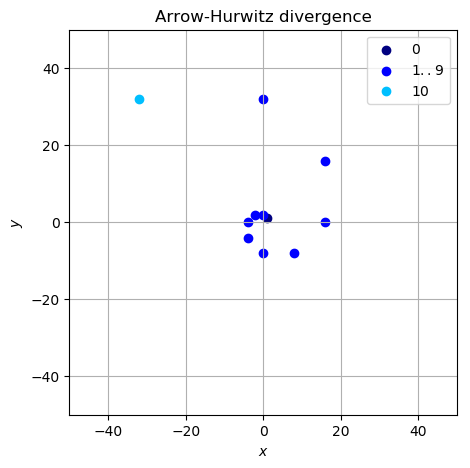
\includegraphics{img/arrow-hurwitz-divergence.png}
    \end{figure}

    Вони, очевидно, розбігаються, хоча здавалося що ми рухаємося у напрямку правильних градєнтів по кожній з компонент.

    \begin{remark}
        Для цієї задачі змінний розмір кроку нас не врятує, його зменшення тільки згладить спіраль по якій точки розбігаються.
    \end{remark}

    Окрім емпіричних спостережень, ми можемо явно довести розбіжність, розглянемо для цього $|x_{k+1}|^2 + |y_{k+1}|^2$:
    \begin{multline}
        |x_{k+1}|^2 + |y_{k+1}|^2 = |x_k - \rho_k y_k|^2 + |y_k + \rho_k x_k|^2 = \\
        = |x_k|^2 + \rho_k^2 \left( |x_k|^2 + |y_k|^2 \right) + |y_k|^2 > |x_k|^2 + |y_k|^2,
    \end{multline}
    у той час як сідловою точкою, очевидно, є $(0, 0)$.
\end{solution}

\begin{remark}
    Не зважаючи на розбіжність методу Ерроу-Гурвіца на такій простій задачі, Ерроу свого часу був удостоєний Нобелівськиї премії з економіки, за задачі які цим методом можна розв'язати.
\end{remark}

Виникає закономірне зпитання а що ж це за задачі такі. 

\section{Сильно опуклі функції}

Для відповіді на це питання нам доведеться ввести 

\begin{definition}[сильно опуклої функції]
    Функція $f = f(x)$ називається $\mu$-сильно опуклою для деякого $\mu > 0$ якщо
    \begin{equation}
        f(\alpha \cdot x + (1 - \alpha) \cdot y) \le \alpha \cdot f(x) + (1 - \alpha) \cdot f(y) - \mu \cdot \alpha \cdot (1 - \alpha) \cdot \no{x - y}^2.
    \end{equation}
\end{definition}

\begin{example}
    Довільна опукла (у звичайному розумінні) функція є $0$-сильно опуклою.
\end{example}

Про всяк введемо також трохи більш узагальнене

\begin{definition}[сильно опуклої функції]
    Функція $f = f(x)$ називається $g$-сильно опуклою для деякого $\mu > 0$ якщо
    \begin{equation}
        f(\alpha \cdot x + (1 - \alpha) \cdot y) \le \alpha \cdot f(x) + (1 - \alpha) \cdot f(y) - \alpha \cdot (1 - \alpha) \cdot g(\no{x - y}).
    \end{equation}
\end{definition}

Можемо записати також альтернетивне визначення
% (чи то пак критерій\todo{Довести, що це критерій.}) 
$\mu$-сильно опуклості:
\begin{equation}
    f(y) \ge f(x) + \sp{\nabla f(x), y - x} + \mu \cdot \no{x - y}^2.
\end{equation}

\begin{remark}
    Просто цікаво, чи володіють якимись гарними властивостями ``майже опуклі'' функції, тобто $\mu$-опуклі функції з $\mu < 0$.
\end{remark}

Так от виявляється, що для задач із сильно опуклою функцією $f$ метод Ерроу-Гурвіца збігається. \medskip

Доведення наведиться нижче у більш загальному випадку, а поки що останннє
\begin{remark}
    Існують певні ергодичні теореми, які стверджують збіжність середнього значення 
    \begin{equation}
        \left(\tilde x_n, \tilde y_n\right) = \left( \frac{x_0 + \ldots + x_n}{n + 1}, \frac{y_0 + \ldots + y_n}{n + 1} \right)
    \end{equation}
    до якоїсь сідлової точки $(\bar x, \bar y)$, але подібні усереднені методи не є практичними, адже вони збігаються дуже повільно, а у задачі вище вже за тисячу ітерацій числа стають настільки великі що машинні похибки ``переважають'' усю теорію.
\end{remark}

\section{Монотонні оператори}

Нагадаємо, що ми намгаємося знайти точку $x \in C$ яка задовольняє варіаційній нерівності
\begin{equation}
    \sp{A x, y - x} \ge 0 \quad \forall y \in C,
\end{equation}
де оператор $A$, взагалі кажучи, не нерозтягуючий. \medskip

Подивимося
% \todo{Показати еквівалентність.}
на цю задачу як на задачу знаходження нерухомої точки оператора
\begin{equation}
    T: x \mapsto P_C \left( x - \rho A x \right),
\end{equation}
де $\rho > 0$. Одразу зауважимо, що ці міркування приводять нас до натсупного алгоритму
\begin{equation}
    x_{k + 1} \coloneqq P_C \left( x_k - \rho_k A x_k \right),
\end{equation} 
збіжність якого ми зараз і проаналізуємо. \medskip

Взагалі хотілося б\footnote{Відомо багато теорем щодо збіжності описаного алгоритму за таких умов.} щоб оператор $T$ був нерозтягуючим. Маємо:
\begin{multline}
    \no{T x - T y}^2 \le \no{x - y - \rho (A x - A y)}^2 \le \\
    \le \no{x - y}^2 - 2 \rho \sp{A x - A y, x - y} + \rho^2 \no{A x - Ay}^2.
\end{multline}

Для подальших оцінок нам знадобиться поняття монотонного оператора.

\begin{definition}[монотонного оператора]
    Оператор $A$: $H \to H$ називається \textit{монотонним} якщо
    \begin{equation}
        \sp{A x - A y, x - y} \ge 0 \quad \forall x \; \forall y.
    \end{equation}
\end{definition}

Поняття монотонності для операторів відіграє схожу роль з поняттям монотонності функцій.

\begin{example}
    Оператор $A$ називається \textit{опуклим} якщо його градієнт $\nabla A$ монотонний.
\end{example}

Аналогічно до $\mu$-сильно опуклих функцій існуюють $\mu$-сильно опуклі оператори, для визначення яких вводиться
\begin{definition}[сильно монотонного оператора]
    Оператор $A$: $H \to H$ називається \textit{$\mu$-сильно монотонним} зі сталою $\mu > 0$ якщо
    \begin{equation}
        \sp{A x - A y, x - y} \ge \mu \cdot \no{x - y}^2 \quad \forall x \; \forall y.
    \end{equation}
\end{definition}

Якщо оператор $A$ --- $\mu$-сильно монотонний то можемо продовжити ланцюжок оцінок:
\begin{multline}
    \no{x - y}^2 - 2 \rho \sp{A x - A y, x - y} + \rho^2 \no{A x - Ay}^2 \le \\
    \le \no{x - y}^2 - 2 \rho \mu \no{x - y}^2 + \rho^2 \no{A x - A y}^2.
\end{multline}

Якщо ж при цьому оператор $A$ ще й $L$-ліпшицевий\footnote{Ліпшицевий з константою $L$, тобто $\no{A x - A y} \le L \cdot \no{x - y}$.}, то можемо продовжити ще:
\begin{multline}
    \no{x - y}^2 - 2 \rho \mu \no{x - y}^2 + \rho^2 \no{A x - A y}^2 \le \\
    \le \no{x - y}^2 - 2 \rho \mu \no{x - y}^2 + \rho^2 L^2 \no{x - y}^2 = \\
    = (1 - 2 \rho \mu + \rho^2 L^2) \no{x - y}^2 = \kappa(\rho) \cdot \no{x - y}^2.
\end{multline}

тобто достатньо обрати $\rho$ так, щоб $\kappa(\rho) \in (0, 1)$. \medskip

Розв'язуючи отриману квадратну нерівність знаходимо:
\begin{equation}
    \rho \in \left(0, \frac{2 \mu}{L^2}\right),
\end{equation}
тобто знайшли цілий інтервал значень $\rho$ для яких наш алгоритм буде збіжним. \medskip

Здавалося б все добре, але подивимося, у якій точці досягається мінімум $\kappa(\rho)$:
\begin{equation}
    \tilde \rho = \frac{\mu}{L^2},
\end{equation}
і чому він дорівнює:
\begin{equation}
    \kappa(\tilde \rho) = 1 - 2 \rho \mu + \rho^2 L^2 = 1 - 2 \frac{\mu}{L^2} \mu + \left( \frac{\mu}{L^2} \right)^2 L^2 = 1 - \frac{\mu^2}{L^2}.
\end{equation}

\begin{remark}
    На жаль, правда життя така, що $\mu$ зазвича доволі мале, а $L$ навпаки --- доволі велике, тому $\rho < 1$ але зовсім трохи. А це у свою чергу означає повільну збіжність.
\end{remark}

\section{Регуляризація}

У той же час майже довільну опуклу функцію $f$ можна замінити\footnote{Цей процес називається регуляризацією.} на $\epsilon$-сильно опуклу функцію $f_\epsilon = f + \epsilon\no{x}^2$, тому може здатися, що всі наші роблеми розв'язані. \medskip

Так, у загальному випадку для монотонного оператора $A$ можна розглянути оператор $A_\epsilon = A + \epsilon {\bf 1}$, де ${\bf 1}$, $x \mapsto x$ --- \emph{одиничний} (\emph{тотожний}) \emph{оператор}. Тоді можемо записати
\begin{equation}
    \sp{A_\epsilon x - A_\epsilon y, x - y} = \underset{\le 0}{\underbrace{\sp{A x - A y, x - y}}} + \epsilon \cdot \no{x - y}^2 \ge \epsilon \cdot \no{x - y}^2,
\end{equation}
тобто оператор $A_\epsilon$ є $\epsilon$-сильно опуклим. \medskip

Це наштовхує на думки про побудову алгоритму з ітераціями вигляду
\begin{equation}
    x_{k + 1} \coloneqq P_C \left( x_k - \rho_k A_{\epsilon_k} x_k \right),
\end{equation}
але тоді постає ще ряд запитань, наприклад які умови мають задовольняти $\{\rho_k\}_{k = 1}^\infty$ і $\{\epsilon_k\}_{k = 1}^\infty$ для збіжності цього алгоритму. Поки що ці запитання лишаємо без відповіді.

\section{Зв'язок із мережевими іграми і рівновагою Неша}

\emph{Цей розділ взято з доповіді} \href{https://simons.berkeley.edu/talks/asu-ozdaglar-3-28-18}{[Asu \"Ozdaglar, 2018]}. \medskip

У багатьох соціальних та економіних задачах, рішення окремих індивідів (агентів) залежать лише від дій їхніх друзів, колег, однолітків чи суперників. Як приклади можна навести:
\begin{itemize}
    \item Поширення інновацій, стилю життя.
    \item Формування громадських думок і соціальне навчання.
    \item Суперництво між конкурентними фірмами.
    \item Забезпечення суспільних благ.
\end{itemize}

Такі взаємодії можна промоделювати мережевою грою, що означає виконання наступних припущень:
\begin{itemize}
    \item Агенти взаємодіють по ребрам мережі, представленої графом.
    \item Виграш кожного гравця залежить від його власних дій і від \emph{агрегованого} значення дій агентів у його околі.
\end{itemize}

Формальніше, модель мережевої гри наступна: $n$ агентів взаємодіють по мережі $G \in \RR^{n \times n}$:
\begin{equation}
    \begin{cases}
        G_{i,j} > 0 & \text{вплив }j\text{ на }i, \\
        G_{i,i} = 0 & \text{без петель}.
    \end{cases}
\end{equation}

У кожного агента $i$ є:
\begin{itemize}
    \item стретегія $x^i \in \mathcal{X}^i$, де $\mathcal{X}^i \subset \RR^n$ --- допустима множина стратегій ;
    \item цільова функція $J^i(x^i, z^i(x)): \RR^n \times \RR^n \to \RR$, де $z^i(x) \coloneqq \sum_{j = 1}^n G_{i,j} x^j$ --- агрегатор.
\end{itemize}

Кожен агент намагється навчитися обчислювати свою оптимальну відповідь:
\begin{equation}
    x_\text{br}^i(z^i) \coloneqq \Argmin_{x^i \in \mathcal{X}^i} J^i(x^i, z^i).
\end{equation}

Нагадаємо
\begin{definition}[рівноваги за Нешем]
    Множина стратегій $\{\bar x_i\}_{i = 1}^n$ називається \emph{рівновагою за Нешем} якщо для кожного гравця $i$, $\bar x^i \in \mathcal{X}^i$:
    \begin{equation}
        J^i \left( \bar x^i, \sum_{j = 1}^n G_{i,j} \bar x^j \right) \le J^i \left( x^i, \sum_{j = 1}^m G_{i,j} \bar x^i \right), \quad \forall x^i \in \mathcal{X}^i.
    \end{equation}
\end{definition}

Можна показати, що при виконанні наступних припущень:
\begin{itemize}
    \item $\mathcal{X}^i \subset \RR^n$ --- замкнені, опуклі та обмежені;
    \item $J^i(x^i, z^i(x))$ опукла по $x^i$, для кожного вектора доповнюючих стратегій $x^{-i} \in \mathcal{X}^{-i}$;
    \item $J^i(x^i, z^i) \in C^2$ по $x^i$ і $z^i$.
\end{itemize}
справджується наступне
\begin{proposition}
    $\bar x$ є рівновагою за Нешем $\iff$ $\bar x$ є розв'язком варіаційної нерівності із допустимою множиною $\mathcal{X}$ і функцією $F$ визначеними наступним чином:
    \begin{align}
        \mathcal{X} &\coloneqq \mathcal{X}^1 \times \dots \times \mathcal{X}^n; \\
        F(x) &\coloneqq [F^i(x)]_{i = 1}^n \coloneqq \begin{bmatrix}
            \nabla_{x^1} J^1(x^1, z^1(x)) \\
            \vdots \\
            \nabla_{x^n} J^n(x^n, z^n(x)) 
        \end{bmatrix}
    \end{align}
\end{proposition}

\begin{proposition}[Facchinei та Pang, 2003]
    Якщо окрім цього, якобіан гри $F$ строго монотонний, то рівновага за Нешем існує та єдина.
\end{proposition}

\section{Подальші припущення}

Надалі будемо розв'язувати наступну задачу:
\begin{equation}
    \label{eq:variational-inequality}
    \text{знайти } x \in C: \quad \sp{A x, y - x} \ge 0, \quad \forall y \in C. 
\end{equation}

Також будемо вважати, що виконані наступні умови:
\begin{itemize}
    \item множина $C \subseteq H$ --- опукла і замкнена;
    \item оператор $A: H \to H$ --- монотонний і ліпшицевий ($L$ --- константа Ліпшиця);
    \item множина розв'язків \eqref{eq:variational-inequality} непорожня.
\end{itemize}


\chapter{Алгоритми}
\section{Класичні алгоритми}

Серед численних алгоритмів розв'язування \eqref{eq:variational-inequality} розглянемо три базових:

\begin{algorithm}[Корпелевич]
    \label{algo:korpelevich}
    \textbf{Ініціалізація.} Вибираємо елементи $x_1$, $\lambda \in \left( 0, \frac{1}{L} \right)$. Покладаємо $n = 1$. \medskip

    \textbf{Крок 1.} Обчислюємо
    \begin{equation}
        y_n = P_C (x_n - \lambda A x_n).
    \end{equation}
    
    Якщо $x_n = y_n$ то зупиняємося і $x_n$ --- розв'язок, інакше переходимо на \medskip
    
    \textbf{Крок 2.} Обчислюємо
    \begin{equation}
        x_{n + 1} = P_C (x_n - \lambda A y_n),
    \end{equation}
    покладаємо $n \coloneqq n + 1$ і переходимо на \textbf{Крок 1.}
\end{algorithm}

\begin{algorithm}[P. Tseng]
    \label{algo:tseng}
    \textbf{Ініціалізація.} Вибираємо елементи $x_1$, $\lambda \in \left( 0, \frac{1}{L} \right)$. Покладаємо $n = 1$. \medskip

    \textbf{Крок 1.} Обчислюємо
    \begin{equation}
        y_n = P_C (x_n - \lambda A x_n).
    \end{equation}
    
    Якщо $x_n = y_n$ то зупиняємося і $x_n$ --- розв'язок, інакше переходимо на \medskip
    
    \textbf{Крок 2.} Обчислюємо
    \begin{equation}
        x_{n + 1} = y_n - \lambda (A y_n - A x_n),
    \end{equation}
    покладаємо $n \coloneqq n + 1$ і переходимо на \textbf{Крок 1.}
\end{algorithm}

\begin{algorithm}[Попов]
    \label{algo:popov}
    \textbf{Ініціалізація.} Вибираємо елементи $x_1$, $y_0$, $\lambda \in \left( 0, \frac{1}{3L} \right)$. Покладаємо $n = 1$. \medskip

    \textbf{Крок 1.} Обчислюємо
    \begin{equation}
        y_n = P_C (x_n - \lambda A y_{n - 1}).
    \end{equation}
    
    \textbf{Крок 2.} Обчислюємо
    \begin{equation}
        x_{n + 1} = P_C (x_n - \lambda A y_n).
    \end{equation}
    
    Якщо $x_{n + 1} = x_n = y_n$ то зупиняємо алгоритм і $x_n$ --- розв'язок, інакше покладаємо $n \coloneqq n + 1$ і переходимо на \textbf{Крок 1.}
\end{algorithm}

\begin{remark}
    У наведеному вище вигляді алгоритми Tseng'a і Попова обчислюють оператор $A$ тричі і двічі на кожну ітерацію відповідно. На цьому можна заощадити якщо кешувати обчислення оператора $A$. У випадку алгоритма Tseng'a спосіб кешування очевидний: один раз обчислюємо $A x_n$ і двічі використовуємо його (для $y_n$ та $x_{n + 1}$). У випадку алгоритма Попова кешування допомагає за рахунок того, що значення $A y_n$ використовується один раз на ітерації $n$ для обчислення $x_{n + 1}$, і ще раз на ітерації $n + 1$ для обчислення значення $y_{n + 1}$. \medskip
    
    В теорії, у випадку коли $P_C$ обчислювати дешево (наприклад, коли це можливо аналітично), а $A$ обчислювати дорого, такий трюк допомагає пришвидшити алгоритм Tseng'a у 1.5, а алгоритм Попова --- у 2 рази.
\end{remark}


\section{Адаптивні алгоритми}

Не так давно з'явилися адаптивні алгоритми, тобто такі, що не вимагають знання константи Ліпшиця. Наведемо адаптивні версії розгялнутих раніше алгоритмів:

\begin{algorithm}[Адаптивний Корпелевич]
    \label{algo:adapt-korpelevich}
    \textbf{Ініціалізація.} Вибираємо елементи $x_1$, $\tau \in (0, 1)$, $\lambda \in (0, +\infty)$. Покладаємо $n = 1$. \medskip

    \textbf{Крок 1.} Обчислюємо
    \begin{equation}
        y_n = P_C (x_n - \lambda A x_n).
    \end{equation}
    
    Якщо $x_n = y_n$ то зупиняємося і $x_n$ --- розв'язок, інакше переходимо на \medskip
    
    \textbf{Крок 2.} Обчислюємо
    \begin{equation}
        x_{n + 1} = P_C (x_n - \lambda A y_n).
    \end{equation}
    
    \textbf{Крок 3.} Обчислюємо
    \begin{equation}
        \lambda_{n + 1} = \begin{cases}
            \lambda_n, \text{ якщо } \sp{A x_n - A y_n, x_{n + 1} - y_n} \le 0, \\
            \min \left\{ \lambda_n, \dfrac{\tau}{2} \dfrac{\no{x_n - y_n}^2 + \no{x_{n + 1} - y_n}^2}{\sp{A x_n - A y_n, x_{n + 1} - y_n}} \right\}, \text{ інакше}.
        \end{cases}
    \end{equation}
    покладаємо $n \coloneqq n + 1$ і переходимо на \textbf{Крок 1.}
\end{algorithm}

\begin{remark}
    У алгоритмі \ref{algo:adapt-korpelevich} можна робити і так:
        \begin{equation}
            \lambda_{n + 1} = \begin{cases}
                \lambda_n, \text{ якщо } A x_n - A y_n = 0, \\
                \min \left\{ \lambda_n, \tau \dfrac{\no{x_n - y_n}}{\no{A x_n - A y_n}} \right\}, \text{ інакше}.
            \end{cases}
        \end{equation}
\end{remark}

\begin{algorithm}[Адаптивний Tseng]
    \label{algo:adapt-tseng}
    \textbf{Ініціалізація.} Вибираємо елементи $x_1$, $\tau \in (0, 1)$, $\lambda \in (0, +\infty)$. Покладаємо $n = 1$. \medskip

    \textbf{Крок 1.} Обчислюємо
    \begin{equation}
        y_n = P_C (x_n - \lambda A x_n).
    \end{equation}
    
    Якщо $x_n = y_n$ то зупиняємося і $x_n$ --- розв'язок, інакше переходимо на \medskip
    
    \textbf{Крок 2.} Обчислюємо
    \begin{equation}
        x_{n + 1} = y_n - \lambda (A y_n - A x_n),
    \end{equation}
    
    \textbf{Крок 3.} Обчислюємо
    \begin{equation}
        \lambda_{n + 1} = \begin{cases}
            \lambda_n, \text{ якщо } A x_n - A y_n = 0, \\
            \min \left\{ \lambda_n, \tau \dfrac{\no{x_n - y_n}}{\no{A x_n - A y_n}} \right\}, \text{ інакше}.
        \end{cases}
    \end{equation}
    покладаємо $n \coloneqq n + 1$ і переходимо на \textbf{Крок 1.}
\end{algorithm}

\begin{algorithm}[Адаптивний Попов]
    \label{algo:adapt-popov}
    \textbf{Ініціалізація.} Вибираємо елементи $x_1$, $y_0$, $\tau \in (0, \frac{1}{3})$, $\lambda \in (0, +\infty)$. Покладаємо $n = 1$. \medskip

    \textbf{Крок 1.} Обчислюємо
    \begin{equation}
        y_n = P_C (x_n - \lambda A y_{n - 1}).
    \end{equation}
        
    \textbf{Крок 2.} Обчислюємо
    \begin{equation}
        x_{n + 1} = P_C (x_n - \lambda A y_n).
    \end{equation}
    
    Якщо $x_{n + 1} = x_n = y_n$ то зупиняємо алгоритм і $x_n$ --- розв'язок, інакше переходимо на \medskip
    
    \textbf{Крок 3.} Обчислюємо
    \begin{equation}
        \lambda_{n + 1} = \begin{cases}
            \lambda_n, \text{ якщо } \sp{A y_{n - 1} - A y_n, x_{n + 1} - y_n} \le 0, \\
            \min \left\{ \lambda_n, \dfrac{\tau}{2} \dfrac{\no{y_{n- 1} - y_n}^2 + \no{x_{n + 1} - y_n}^2}{\sp{A y_{n - 1} - A y_n, x_{n + 1} - y_n}} \right\}, \text{ інакше}.
        \end{cases}
    \end{equation}
    покладаємо $n \coloneqq n + 1$ і переходимо на \textbf{Крок 1.}
\end{algorithm}

\begin{remark}
    У алгоритмі \ref{algo:adapt-popov} можна робити і так:
        \begin{equation}
            \lambda_{n + 1} = \begin{cases}
                \lambda_n, \text{ якщо } A y_{n - 1} - A y_n = 0, \\
                \min \left\{ \lambda_n, \tau \dfrac{\no{y_{n - 1} - y_n}}{\no{A y_{n - 1} - A y_n}} \right\}, \text{ інакше}.
            \end{cases}
        \end{equation}
\end{remark}


\section{Алгоритм Маліцького---Tam'a}

Зовсім нещодавно (у 2015-ому році) Юра Маліцький запропонував наступну схему:

\begin{algorithm}[Маліцький---Tam]
    \label{algo:malitsky-tam}
    \textbf{Ініціалізація.} Вибираємо елементи $x_1, x_0 \in H$, $\lambda \in (0, \frac{1}{2L})$. Покладаємо $n = 1$. \medskip

    \textbf{Крок.} Обчислюємо
    \begin{equation}
        x_{n + 1} = P_C (x_n - \lambda A x_n - \lambda (A x_n - A x_{n - 1})).
    \end{equation}
    
    Якщо $x_{n + 1} = x_n = x_{n - 1}$ то зупиняємо алгоритм і $x_n$ --- розв'язок, інакше покладаємо $n \coloneqq n + 1$, і повторюємо
\end{algorithm}

\begin{algorithm}[Адаптивний Маліцький---Tam]
    \label{algo:adapt-malitsky-tam}
    \textbf{Ініціалізація.} Вибираємо елементи $x_1, x_0 \in H$, $\lambda_1, \lambda_0 > 0$, $\tau \in (0, \frac{1}{2})$. Покладаємо $n = 1$. \medskip

    \textbf{Крок 1.} Обчислюємо
    \begin{equation}
        x_{n + 1} = P_C (x_n - \lambda A x_n - \lambda (A x_n - A x_{n - 1})).
    \end{equation}
    
    Якщо $x_{n + 1} = x_n = x_{n - 1}$ то зупиняємо алгоритм і $x_n$ --- розв'язок, інакше переходимо на \medskip

    \textbf{Крок 2.} Обчислюємо
    \begin{equation}
        \lambda_{n + 1} = \min \left\{ \lambda_ n, \tau  \frac{\|x_{n + 1} - x_n\|}{\|A x_{n + 1} - A x_n} \right\},
    \end{equation}
    покладаємо $n \coloneqq n + 1$ і переходимо на \textbf{Крок 1.}
\end{algorithm}


\chapter{Задачі}
Для порівняння алгоритмів нам знадобляться тестові задачі різної складності та різних розмірів. У якості таких задачі розглянемо:

\section{Перша задача}

Класичний приклад. Допустимою множиною є увесь простір: $C = \RR^m$, а $F(x) = Ax$, де $A$ --- квадратна $m \times m$ матриця, елементи якої визначаються наступним чином:
\begin{equation}
    a_{i,j} = \begin{cases}
        -1, & j = m - 1 - i > i, \\
        1, & j = m - 1 - i < i, \\
        0, & \text{інакше}.
    \end{cases}
\end{equation}

\begin{remark}
    Тут і надалі нуметрація рядків/стовпчиків матриць, а також елементів масивів починається з нуля. Якщо у вашій мові програмування нумерація починається з одиниці то у виразах вище замість $m - 1$ має бути $m + 1$.
\end{remark}

Це визначає матрицю, чия бічна діагональ складається з половини одиниць і половини мінус одиниць, а решта елементів якої нульові. Для наглядності наведемо кілька преших матриць, для $m = 2, 4$:
\begin{equation}
    \begin{pmatrix}
        0 & -1 \\
        1 & 0
    \end{pmatrix}
    \qquad
    \begin{pmatrix}
        0 & 0 & 0 & -1 \\
        0 & 0 & -1 & 0 \\
        0 & 1 & 0 & 0 \\
        1 & 0 & 0 & 0
    \end{pmatrix}
    % \qquad
    % \begin{pmatrix}
    %     0 & 0 & 0 & 0 & 0 & -1 \\
    %     0 & 0 & 0 & 0 & -1 & 0 \\
    %     0 & 0 & 0 & -1 & 0 & 0 \\
    %     0 & 0 & 1 & 0 & 0 & 0 \\
    %     0 & 1 & 0 & 0 & 0 & 0 \\
    %     1 & 0 & 0 & 0 & 0 & 0
    % \end{pmatrix}
\end{equation}

Для парних $m$ нульовий вектор є розв'язком відповідної варіаційної нерівності \eqref{eq:variational-inequality}. Для усіх чисельних еспериментів ми брали $x_0 = (1, \dots, 1)$, $\epsilon = 10^{-3}$, $\lambda = 0.4$. 

\begin{remark}
    Ця задача є узагальненням \ref{classical-example}. Як ми вже знаємо, звичайні градієнтні методи для неї не збігаються.
\end{remark}

\begin{remark}
    Для цієї задачі $P_C = \text{Id}$, а тому алгоритми Корпелевич і Tseng'a еквівалентні. Втім, некешована версія алгоритму Tseng'a буде працювати повільніше, у чому ми переконаємося у результатах.
\end{remark}

\section{Друга задача}

Візьмемо $F(x) = M x + q$, де випадкова матриця $M$ генерується наступним чином:
\begin{equation}
    M = A A^\intercal + B + D,
\end{equation}
де всі елементи $m \times m$ матриці $A$ і $m \times m$ кососиметричної матриці $B$ обираються рівномірно випадково з $(-5, 5)$, а усі елементи діагональної матриці $D$ вибираються рівномірно випадково з $(0, 0.3)$ (як наслідок, матриця $M$ додатно визначена), а кожен елемент $q$ обирається рівномірно випадково з $(-500, 0)$. Допустимою множиною є 
\begin{equation}
    C = \left\{ x \in \RR_+^m \middle| x_1 + x_2 + \dots + x_m = m \right\}.
\end{equation}

Допустима множина цієї задачі --- так званий \emph{probability symplex} (з точністю до константи $m$). Для проектування $\vec y$ на нього ми використовували наступний явний
\begin{algorithm}\nothing

    \textbf{Крок 1.} Відсортувати елементи $\vec y$ і зберегти в $\vec u$: $u_1 \ge \dots \ge u_m$. \medskip
        
    \textbf{Крок 2.} Знайти $k = \max j$: $u_j + \frac{1}{j} \left( m - \Sum_{i = 1}^j u_i \right) > 0$. \medskip
        
    \textbf{Крок 3.} Видати вектор з елементами $x_i = \max\{y_i + \lambda, 0\}$, $\lambda = \frac{1}{k} \left( m - \Sum_{i = 1}^k u_i \right)$.
\end{algorithm}

\emph{Цей алгоритм взято із статті \cite{duchi-et-al}}. \medskip

Для усіх чисельних експериментів ми брали $x_0 = (1, \dots, 1)$, $\epsilon = 10^{-3}$, $L = \no{M}$. також, для кожного розмірку задачі було згенеровано кілька різних $M$.

\section{Третя задача}

Нелінійна доповлююча задача Коджими---Шиндо була розглянута у \cite{pang-gabriel} і \cite{kanzow}, де $m = 4$, а функція $F$ визначається наступним чином:
\begin{equation}
    F(x_1, x_2, x_3, x_4) = \begin{bmatrix}
        3 x_1^2 + 2 x_1 x_2 + 2 x_2^2 + x_3 + 3 x_4 - 6 \\
        2 x_1^2 + x_1 + x_2^2 + 10 x_3 + 2 x_4 - 2 \\
        3 x_1^2 + x_1 x_2 + 2 x_2^2 + 2 x_3 + 9 x_4 - 9 \\
        x_1^2 + 3 x_2^2 + 2 x_3 + 3 x_4 - 3
    \end{bmatrix}.
\end{equation}

Допустимою множиною знову є ймовірнісний симплекс \[C = \left\{ x \in \RR^4 \middle| x_1 + x_2 + x_3 + x_4 \right\}.\] Для чисельних експериментів ми спершу взяли кілька конкретних стартових точок $x_1 = (1, 1, 1, 1)$ і $x_1 = (0.5, 0.5, 2, 1)$, а потім ще декілька випадкових точок із $C$. Для усіх стартових точок проводилося два тести: один із $\epsilon = 10^{-3}$, второй с $\epsilon = 10^{-6}$.

\begin{remark}
    У цієї задачі неєдиний розв'язок, хоча здебільшого алгоритми збігалися до $x_\star = (1.225, 0, 0, 2.775)$. Втім, не завжди, що і пояснює значну різницю у кількості ітерацій між деякими алгоритмами на деяких тестах.
\end{remark}

\section{Четверта задача}

Цей приклад був розглянутий Суном у \cite{sun}:
\begin{equation}
    \begin{aligned}
        F(x) &= F_1(x) + F_2(x), \\
        F_1(x) &= (f_1(x), f_2(x), \dots, f_m(x)), \\
        F_2(x) &= D x + c, \\
        f_i(x) &= x_{i - 1}^2 + x_i^2 + x_{i - 1} x_i + x_i x_{i + 1}, \quad m = 1, 2, \dots, m, \\
        x_0 &= x_{m + 1} = 0,
    \end{aligned}
\end{equation}
де $D$ --- квадратна $m \times m$ матриця з наступними елементами:
\begin{equation}
    d_{i,j} = \begin{cases}
         1, & j = i - 1, \\
         4, & j = i, \\
        -2, & j = i + 1, \\
         0, & \text{інакше},
    \end{cases}
\end{equation}
$c = (-1, -1, \dots, -1)$. Допустимою множиною є $C = \RR_+^m$, а початкова точка $x_1 = (0, 0, \dots, 0)$. \medskip

Для кращого розуміння наведемо матрицю $D$ для кількох перших $m = 3, 4, 5$:
\begin{equation}
    \begin{pmatrix}
        4 & -2 &  0 \\
        1 &  4 & -2 \\
        0 &  1 &  4
    \end{pmatrix}
    \qquad
    \begin{pmatrix}
        4 & -2 &  0 &  0 \\
        1 &  4 & -2 &  0 \\
        0 &  1 &  4 & -2 \\
        0 &  0 &  1 &  4
    \end{pmatrix}
    \qquad
    \begin{pmatrix}
        4 & -2 &  0 &  0 &  0 \\
        1 &  4 & -2 &  0 &  0 \\
        0 &  1 &  4 & -2 &  0 \\
        0 &  0 &  1 &  4 & -2 \\
        0 &  0 &  0 &  1 &  4
    \end{pmatrix}
\end{equation}

Для усіх чисельних експериментів ми брали $x_1 = (0, \dots, 0)$. Знову ж таки, було розглянуто два значення $\epsilon$: $10^{-3}$ і $10^{-6}$.

\begin{remark}
    Матриця тридіагональна, ми цим скористаємося для ефективного зберігання і множення.
\end{remark}


\begin{landscape}
\chapter{Результати}
Тестування відбувалося на машині із процесором Intel Core i7-8550U 1.99GHz під 64-бітною версією операційної системи Windows 10.

\section{Перша задача, неадаптивні алгоритми}

\begin{table}[H]
    \centering
    \begin{tabular}{||c||c|c||c|c|c|c||c|c|c|c||c|c|c|c||} \hline \hline
        \multirow{2}{*}{$m$} & \multicolumn{2}{c||}{Корп.} & \multicolumn{2}{c|}{Tseng} & \multicolumn{2}{c||}{кеш. Tseng} & \multicolumn{2}{c|}{Попов} & \multicolumn{2}{c||}{кеш. Попов} & \multicolumn{2}{c|}{Маліц.} & \multicolumn{2}{c||}{кеш. Маліц.} \\ \cline{2-15}
         & час & ітер. & час & ітер. & час & ітер. & час & ітер. & час & ітер. & час & ітер. & час & ітер. \\ \hline \hline
        1000 & 0.10 & 132 & 0.11 & 132 & 0.08 & 132 & 0.05 & 89 & 0.03 & 89 & 0.08 & 91 & 0.03 & 91 \\ \hline
        2000 & 0.58 & 137 & 0.92 & 137 & 0.53 & 137 & 0.36 & 92 & 0.18 & 92 & 0.54 & 94 & 0.19 & 94 \\ \hline
        5000 & 4.08 & 144 & 6.39 & 144 & 4.34 & 144 & 2.85 & 96 & 1.46 & 96 & 4.37 & 98 & 1.53 & 98 \\ \hline
        10000 & 17.43 & 148 & 26.73 & 148 & 17.82 & 148 & 13.14 & 99 & 6.56 & 99 & 18.94 & 101 & 5.85 & 101 \\ \hline
        \hline
    \end{tabular}
    \caption{Результати  неадаптивних алгоритмів для першої задачі}
    \label{tab:1}
\end{table}

Бачимо що алгоритм Корпелевич і кешований алгоритм Tseng'a справді показують майже однакові результати, що є непрямим доказом їхньої еквівалентності. Однакова кількість ітерацій некешованих і кешованих версій усіх алгоритмів слугує непрямим доказом їхньої еквівалентності. Втім, кешовані версії передбачувано виграють (у 1.5--3 рази) у некешованих версій по часу роботи. З точки зору часу роботи найкращі результати показує кешована версія алгоритму Маліцького---Tam'a, з точки зору числа ітерацій --- алгоритм Попова, хоча алгоритм Маліцького---Tam'a майже йому не поступається.

\section{Перша задача, адаптивні алгоритми}

\begin{table}[H]
    \centering
    \begin{tabular}{||c||c|c|c|c||c|c|c|c||c|c|c|c||c|c|c|c||} \hline \hline
        \multirow{2}{*}{$m$} & \multicolumn{2}{c|}{Корп.} & \multicolumn{2}{c||}{кеш. Корп.} & \multicolumn{2}{c|}{Tseng} & \multicolumn{2}{c||}{кеш. Tseng} & \multicolumn{2}{c|}{Попов} & \multicolumn{2}{c||}{кеш. Попов} & \multicolumn{2}{c|}{Маліц.} & \multicolumn{2}{c||}{кеш. Маліц.} \\ \cline{2-17}
         & час & ітер. & час & ітер. & час & ітер. & час & ітер. & час & ітер. & час & ітер. & час & ітер. & час & ітер. \\ \hline \hline
        1000 & 0.26 & 132 & 0.07 & 132 & 0.24 & 132 & 0.08 & 132 & 0.13 & 89 & 0.04 & 89 & 0.17 & 91 & 0.03 & 91 \\ \hline
        2000 & 1.74 & 137 & 0.57 & 137 & 2.01 & 137 & 0.57 & 137 & 1.09 & 92 & 0.19 & 92 & 1.39 & 94 & 0.24 & 94 \\ \hline
        5000 & 12.66 & 144 & 4.29 & 144 & 15.40 & 144 & 4.24 & 144 & 8.16 & 96 & 1.38 & 96 & 10.25 & 98 & 1.65 & 98 \\ \hline
        10000 & 51.37 & 148 & 17.61 & 148 & 66.98 & 148 & 17.16 & 148 & 34.25 & 99 & 5.85 & 99 & 40.75 & 101 & 5.84 & 101 \\ \hline
        \hline
    \end{tabular}
    \caption{Результати адаптивних алгоритмів для першої задачі}
    \label{tab:1-adapt}
\end{table}

Бачимо що алгоритм Корпелевич і алгоритм Tseng'a справді показують майже однакові результати, що є непрямим доказом їхньої еквівалентності. Однакова кількість ітерацій некешованих і кешованих версій усіх алгоритмів слугує непрямим доказом їхньої еквівалентності. Втім, кешовані версії передбачувано виграють (у 3--7 разів) у некешованих версій по часу роботи. З точки зору часу роботи найкращі і майже еквівалентні результати показують кешовані версії алгоритмів Маліцького---Tam'a і Попова, з точки зору числа ітерацій --- алгоритм Попова, хоча алгоритм Маліцького---Tam'a майже йому не поступається.

\section{Перша задача із розрідженими матрицями, неадаптивні алгоритми}

Нескладно помітити, що матриця $A$ дуже розріджена, що наводить на ідею скористатися модулем scipy.sparse для ефективної роботи з розрідженими матрицями. Це дозволить нам розв'язувати задачу для значно більших $m$.

\begin{table}[H]
    \centering
    \begin{tabular}{||c||c|c||c|c|c|c||c|c|c|c||c|c|c|c||} \hline \hline
        \multirow{2}{*}{$m$} & \multicolumn{2}{c||}{Корп.} & \multicolumn{2}{c|}{Tseng} & \multicolumn{2}{c||}{кеш. Tseng} & \multicolumn{2}{c|}{Попов} & \multicolumn{2}{c||}{кеш. Попов} & \multicolumn{2}{c|}{Маліц.} & \multicolumn{2}{c||}{кеш. Маліц.} \\ \cline{2-15}
         & час & ітер. & час & ітер. & час & ітер. & час & ітер. & час & ітер. & час & ітер. & час & ітер. \\ \hline \hline
        50000 & 0.15 & 159 & 0.25 & 159 & 0.16 & 159 & 0.10 & 106 & 0.08 & 106 & 0.13 & 108 & 0.08 & 108 \\ \hline
        100000 & 0.51 & 164 & 0.74 & 164 & 0.39 & 164 & 0.37 & 109 & 0.33 & 109 & 0.43 & 111 & 0.30 & 111 \\ \hline
        200000 & 2.32 & 169 & 3.06 & 169 & 2.53 & 169 & 1.56 & 112 & 1.22 & 112 & 2.13 & 114 & 1.41 & 114 \\ \hline
        500000 & 6.21 & 175 & 8.26 & 175 & 6.87 & 175 & 4.14 & 117 & 3.33 & 117 & 5.74 & 119 & 3.78 & 119 \\ \hline
        \hline
    \end{tabular}
    \caption{Результати неадаптивних алгоритмів для першої задачі із розрідженими матрицями}
    \label{tab:1-sparse}
\end{table}

Бачимо що алгоритм Корпелевич і алгоритм Tseng'a справді показують майже однакові результати, що є непрямим доказом їхньої еквівалентності. Однакова кількість ітерацій некешованих і кешованих версій усіх алгоритмів слугує непрямим доказом їхньої еквівалентності. Тут перевага кешування вже не така очевидна, адже ми значно здешевили обчислення оператора $A$, хоча все ще присутня (у 1.5 рази). З точки зору часу роботи найкращі і майже еквівалентні результати показують кешовані версії алгоритмів Маліцького---Tam'a і Попова, з точки зору числа ітерацій --- алгоритм Попова, хоча алгоритм Маліцького---Tam'a майже йому не поступається.

\section{Перша задача із розрідженими матрицями, адаптивні алгоритми}

\begin{table}[H]
    \centering
    \begin{tabular}{||c||c|c|c|c||c|c|c|c||c|c|c|c||c|c|c|c||} \hline \hline
        \multirow{2}{*}{$m$} & \multicolumn{2}{c|}{Корп.} & \multicolumn{2}{c||}{кеш. Корп.} & \multicolumn{2}{c|}{Tseng} & \multicolumn{2}{c||}{кеш. Tseng} & \multicolumn{2}{c|}{Попов} & \multicolumn{2}{c||}{кеш. Попов} & \multicolumn{2}{c|}{Маліц.} & \multicolumn{2}{c||}{кеш. Маліц.} \\ \cline{2-17}
         & час & ітер. & час & ітер. & час & ітер. & час & ітер. & час & ітер. & час & ітер. & час & ітер. & час & ітер. \\ \hline \hline
        50000 & 0.89 & 159 & 0.61 & 159 & 0.63 & 159 & 0.45 & 159 & 0.53 & 106 & 0.16 & 106 & 0.34 & 108 & 0.15 & 108 \\ \hline
        100000 & 1.53 & 164 & 0.95 & 164 & 1.13 & 164 & 0.54 & 164 & 0.89 & 109 & 0.35 & 109 & 0.75 & 111 & 0.31 & 111 \\ \hline
        200000 & 6.21 & 169 & 3.58 & 169 & 6.18 & 169 & 3.57 & 169 & 4.05 & 112 & 2.00 & 112 & 4.11 & 114 & 2.03 & 114 \\ \hline
        500000 & 16.27 & 175 & 9.29 & 175 & 16.35 & 175 & 9.29 & 175 & 10.96 & 117 & 5.21 & 117 & 11.03 & 119 & 5.22 & 119 \\ \hline
        \hline
    \end{tabular}
    \caption{Результати адаптивних алгоритмів для першої задачі із розрідженими матрицями}
    \label{tab:1-sparse-adapt}
\end{table}

Бачимо що алгоритм Корпелевич і алгоритм Tseng'a справді показують майже однакові результати, що є непрямим доказом їхньої еквівалентності. Однакова кількість ітерацій некешованих і кешованих версій усіх алгоритмів слугує непрямим доказом їхньої еквівалентності. Тут перевага кешування вже не така очевидна, адже ми значно здешевили обчислення оператора $A$, хоча все ще присутня (у 2 рази). З точки зору часу роботи найкращі і майже еквівалентні результати показують кешовані версії алгоритмів Маліцького---Tam'a і Попова, з точки зору числа ітерацій --- алгоритм Попова, хоча алгоритм Маліцького---Tam'a майже йому не поступається.

\section{Друга задача, неадаптивні алгоритми}

\begin{table}[H]
    \centering
    \begin{tabular}{||c||c|c||c|c|c|c||c|c|c|c||c|c|c|c||} \hline \hline
        \multirow{2}{*}{$m$} & \multicolumn{2}{c||}{Корп.} & \multicolumn{2}{c|}{Tseng} & \multicolumn{2}{c||}{кеш. Tseng} & \multicolumn{2}{c|}{Попов} & \multicolumn{2}{c||}{кеш. Попов} & \multicolumn{2}{c|}{Маліц.} & \multicolumn{2}{c||}{кеш. Маліц.} \\ \cline{2-15}
         & час & ітер. & час & ітер. & час & ітер. & час & ітер. & час & ітер. & час & ітер. & час & ітер. \\ \hline \hline
        100 & 0.62 & 967 & 0.48 & 967 & 0.40 & 967 & 0.55 & 967 & 0.43 & 967 & 0.47 & 967 & 0.29 & 967 \\ \hline
        100 & 0.71 & 1151 & 0.58 & 1151 & 0.47 & 1151 & 0.68 & 1151 & 0.58 & 1151 & 0.59 & 1151 & 0.36 & 1151 \\ \hline
        100 & 0.63 & 1086 & 0.54 & 1086 & 0.42 & 1086 & 0.62 & 1086 & 0.50 & 1086 & 0.55 & 1086 & 0.34 & 1086 \\ \hline
        200 & 1.41 & 1849 & 1.07 & 1849 & 0.90 & 1849 & 1.39 & 1849 & 1.26 & 1849 & 1.08 & 1849 & 0.72 & 1849 \\ \hline
        200 & 1.30 & 1672 & 1.01 & 1672 & 0.85 & 1672 & 1.30 & 1672 & 1.10 & 1672 & 1.03 & 1672 & 0.69 & 1672 \\ \hline
        200 & 1.35 & 1715 & 1.13 & 1715 & 0.91 & 1715 & 1.32 & 1715 & 1.16 & 1715 & 1.03 & 1715 & 0.71 & 1715 \\ \hline
        500 & 3.67 & 2523 & 2.34 & 2523 & 2.07 & 2523 & 3.63 & 2523 & 3.30 & 2523 & 2.53 & 2523 & 1.88 & 2523 \\ \hline
        500 & 4.33 & 2543 & 2.74 & 2543 & 2.29 & 2543 & 3.77 & 2543 & 3.27 & 2543 & 2.39 & 2543 & 1.94 & 2543 \\ \hline
        500 & 4.07 & 2725 & 2.62 & 2725 & 2.36 & 2725 & 4.10 & 2725 & 3.48 & 2725 & 2.58 & 2725 & 2.16 & 2725 \\ \hline 
        1000 & 10.09 & 3542 & 8.29 & 3542 & 7.23 & 3542 & 9.62 & 3542 & 8.05 & 3542 & 7.95 & 3543 & 5.07 & 3543 \\ \hline
        1000 & 9.18 & 3570 & 7.37 & 3570 & 6.16 & 3570 & 10.57 & 3570 & 8.05 & 3570 & 7.35 & 3570 & 4.75 & 3570 \\ \hline
        1000 & 9.40 & 3471 & 7.55 & 3471 & 6.67 & 3471 & 9.68 & 3471 & 7.76 & 3471 & 7.34 & 3471 & 5.11 & 3471 \\ \hline
        \hline
    \end{tabular}
    \caption{Результати неадаптивних алгоритмів для другої задачі}
    \label{tab:2}
\end{table}

% У цій задачі основна складність все ще у обчисленні оператора $A$, %($O(m^2)$)
% хоча обчислення проекції вже більш складне, %($O(m \log m)$)
% тому алгоритм Tseng'a має певну перевагу над алгоритмом Попова, який у свою чергу випереджає алгоритм Корпелевич.  Знову ж таки, кешування дає перевагу на великих задачах, хоча вона вже не у 1.5--2 рази.

% Можна додати якийсь із матричних розкладів $M$ для пришвидшення множення $M x$.

\section{Друга задача, адаптивні алгоритми}

\begin{table}[H]
    \centering
    \begin{tabular}{||c||c|c|c|c||c|c|c|c||c|c|c|c||c|c|c|c||} \hline \hline
        \multirow{2}{*}{$m$} & \multicolumn{2}{c|}{Корп.} & \multicolumn{2}{c||}{кеш. Корп.} & \multicolumn{2}{c|}{Tseng} & \multicolumn{2}{c||}{кеш. Tseng} & \multicolumn{2}{c|}{Попов} & \multicolumn{2}{c||}{кеш. Попов} & \multicolumn{2}{c|}{Маліц.} & \multicolumn{2}{c||}{кеш. Маліц.} \\ \cline{2-17}
         & час & ітер. & час & ітер. & час & ітер. & час & ітер. & час & ітер. & час & ітер. & час & ітер. & час & ітер. \\ \hline \hline
        100 & 1.14 & 967 & 0.64 & 967 & 0.99 & 967 & 0.44 & 967 & 0.97 & 967 & 0.51 & 967 & 0.89 & 967 & 0.35 & 967 \\ \hline
        100 & 1.16 & 1151 & 0.73 & 1151 & 1.10 & 1151 & 0.52 & 1151 & 1.15 & 1151 & 0.58 & 1151 & 1.09 & 1151 & 0.42 & 1151 \\ \hline
        100 & 1.10 & 1086 & 0.69 & 1086 & 1.02 & 1086 & 0.49 & 1086 & 1.08 & 1086 & 0.56 & 1086 & 1.01 & 1086 & 0.41 & 1086 \\ \hline
        200 & 2.30 & 1849 & 1.59 & 1849 & 2.01 & 1849 & 1.10 & 1849 & 2.37 & 1849 & 1.56 & 1849 & 2.33 & 1849 & 0.90 & 1849 \\ \hline
        200 & 2.06 & 1672 & 1.38 & 1672 & 1.74 & 1672 & 1.01 & 1672 & 2.06 & 1672 & 1.21 & 1672 & 1.88 & 1672 & 0.81 & 1672 \\ \hline
        200 & 2.07 & 1715 & 1.46 & 1715 & 1.82 & 1715 & 0.94 & 1715 & 2.05 & 1715 & 1.27 & 1715 & 1.83 & 1715 & 0.86 & 1715 \\ \hline
        500 & 5.30 & 2523 & 3.88 & 2523 & 3.85 & 2523 & 2.32 & 2523 & 4.68 & 2523 & 3.25 & 2523 & 3.71 & 2523 & 2.03 & 2523 \\ \hline
        500 & 5.08 & 2543 & 4.13 & 2543 & 3.88 & 2543 & 2.50 & 2543 & 5.14 & 2543 & 3.29 & 2543 & 4.16 & 2543 & 2.14 & 2543 \\ \hline
        500 & 5.36 & 2725 & 3.99 & 2725 & 3.99 & 2725 & 2.43 & 2725 & 5.26 & 2725 & 3.50 & 2725 & 4.15 & 2725 & 2.33 & 2725 \\ \hline
        1000 & 15.93 & 3542 & 10.31 & 3542 & 11.56 & 3542 & 6.54 & 3542 & 14.59 & 3542 & 8.05 & 3542 & 12.11 & 3543 & 5.45 & 3543 \\ \hline
        1000 & 14.28 & 3570 & 9.68 & 3570 & 11.33 & 3570 & 6.51 & 3570 & 15.09 & 3570 & 7.89 & 3570 & 11.13 & 3570 & 4.89 & 3570 \\ \hline
        1000 & 14.43 & 3471 & 9.42 & 3471 & 11.47 & 3471 & 6.40 & 3471 & 14.79 & 3471 & 8.50 & 3471 & 11.99 & 3471 & 5.37 & 3471 \\ \hline
        \hline
    \end{tabular}
    \caption{Результати адаптивних алгоритмів для другої задачі}
    \label{tab:2-adapt}
\end{table}

\section{Третя задача, адаптивні алгоритми}

\begin{table}[H]
    \centering
    \begin{tabular}{||c|c||c|c|c|c||c|c|c|c||c|c|c|c||c|c|c|c||} \hline \hline
        \multirow{2}{*}{$x_1$} & \multirow{2}{*}{$\epsilon$} & \multicolumn{2}{c|}{Корп.} & \multicolumn{2}{c||}{кеш. Корп.} & \multicolumn{2}{c|}{Tseng} & \multicolumn{2}{c||}{кеш. Tseng} & \multicolumn{2}{c|}{Попов} & \multicolumn{2}{c||}{кеш. Попов} & \multicolumn{2}{c|}{Маліц.} & \multicolumn{2}{c||}{кеш. Маліц.} \\ \cline{3-18}
        & & час & ітер. & час & ітер. & час & ітер. & час & ітер. & час & ітер. & час & ітер. & час & ітер. & час & ітер. \\ \hline \hline
        \multirow{2}{*}{$(1, 1, 1, 1)$} & $10^{-3}$ & 0.02 & 30 & 0.01 & 30 & 0.05 & 156 & 0.03 & 156 & 0.01 & 29 & 0.01 & 29 & 0.02 & 49 & 0.01 & 49 \\ \cline{2-18}
        & $10^{-6}$ & 0.02 & 58 & 0.01 & 58 & 0.15 & 475 & 0.08 & 475 & 0.02 & 56 & 0.01 & 56 & 0.04 & 142 & 0.02 & 142 \\ \hline
        \multirow{2}{*}{$(\frac{1}{2}, \frac{1}{2}, 2, 1)$} & $10^{-3}$ & 0.02 & 51 & 0.01 & 51 & 0.33 & 980 & 0.20 & 980 & 0.02 & 51 & 0.01 & 51 & 0.02 & 69 & 0.01 & 69 \\ \cline{2-18}
        & $10^{-6}$ & 0.04 & 104 & 0.03 & 104 & 2.00 & 6503 & 1.13 & 6503 & 0.03 & 104 & 0.02 & 104 & 0.05 & 156 & 0.02 & 156 \\ \hline
        \multirow{2}{*}{random} & $10^{-3}$ & 0.01 & 37 & 0.01 & 37 & 0.14 & 444 & 0.09 & 444 & 0.01 & 36 & 0.01 & 36 & 0.02 & 68 & 0.01 & 68 \\ \cline{2-18}
        & $10^{-6}$ & 0.03 & 72 & 0.02 & 72 & 0.52 & 1602 & 0.31 & 1602 & 0.03 & 71 & 0.02 & 71 & 0.05 & 154 & 0.03 & 154 \\ \hline
        \multirow{2}{*}{random} & $10^{-3}$ & 0.01 & 39 & 0.01 & 39 & 0.12 & 359 & 0.07 & 359 & 0.02 & 55 & 0.01 & 55 & 0.05 & 148 & 0.02 & 148 \\ \cline{2-18}
        & $10^{-6}$ & 0.04 & 121 & 0.03 & 121 & 0.40 & 1231 & 0.24 & 1231 & 0.05 & 141 & 0.03 & 141 & 0.20 & 632 & 0.10 & 632 \\ \hline
        \multirow{2}{*}{random} & $10^{-3}$ & 0.02 & 46 & 0.01 & 46 & 0.37 & 1160 & 0.23 & 1160 & 0.02 & 46 & 0.01 & 46 & 0.02 & 69 & 0.01 & 69 \\ \cline{2-18}
        & $10^{-6}$ & 0.03 & 94 & 0.02 & 94 & --- & --- & --- & --- & 0.03 & 94 & 0.02 & 94 & 0.05 & 165 & 0.02 & 165 \\ \hline    
        \hline
    \end{tabular}
    \caption{Результати адаптивних алгоритмів для третьої задачі}
    \label{tab:3-adapt}
\end{table}


\section{Четверта задача, адаптивні алгоритми}

\begin{table}[H]
    \centering
    \begin{tabular}{||c|c||c|c|c|c||c|c|c|c||c|c|c|c||c|c|c|c||} \hline \hline
        \multirow{2}{*}{$m$} & \multirow{2}{*}{$\epsilon$} & \multicolumn{2}{c|}{Корп.} & \multicolumn{2}{c||}{кеш. Корп.} & \multicolumn{2}{c|}{Tseng} & \multicolumn{2}{c||}{кеш. Tseng} & \multicolumn{2}{c|}{Попов} & \multicolumn{2}{c||}{кеш. Попов} & \multicolumn{2}{c|}{Маліц.} & \multicolumn{2}{c||}{кеш. Маліц.} \\ \cline{3-18}
        & & час & ітер. & час & ітер. & час & ітер. & час & ітер. & час & ітер. & час & ітер. & час & ітер. & час & ітер. \\ \hline \hline

        \hline
    \end{tabular}
    \caption{Результати адаптивних алгоритмів для четвертої задачі}
    \label{tab:4-adapt}
\end{table}

\section{Четверта задача із розрідженими матрицями, адаптивні алгоритми}

\begin{table}[H]
    \centering
    \begin{tabular}{||c|c||c|c|c|c||c|c|c|c||c|c|c|c||c|c|c|c||} \hline \hline
        \multirow{2}{*}{$m$} & \multirow{2}{*}{$\epsilon$} & \multicolumn{2}{c|}{Корп.} & \multicolumn{2}{c||}{кеш. Корп.} & \multicolumn{2}{c|}{Tseng} & \multicolumn{2}{c||}{кеш. Tseng} & \multicolumn{2}{c|}{Попов} & \multicolumn{2}{c||}{кеш. Попов} & \multicolumn{2}{c|}{Маліц.} & \multicolumn{2}{c||}{кеш. Маліц.} \\ \cline{3-18}
        & & час & ітер. & час & ітер. & час & ітер. & час & ітер. & час & ітер. & час & ітер. & час & ітер. & час & ітер. \\ \hline \hline

        \hline
    \end{tabular}
    \caption{Результати адаптивних алгоритмів для четвертої задачі із розрідженими матрицями}
    \label{tab:4-sparse-adapt}
\end{table}

\end{landscape}

\chapter[Висновок]{\MakeUppercase{Висновок}}
В рамках дипломної роботи були виконані наступні завдання:
\begin{enumerate}[label=--]
    \item розглянуто широкий спектр алгоритмів розв'язання варіаційної нерівності: алгоритми Корпелевич, Tseng'a, Попова, Маліцького---Tam'a;
    \item розроблено програмний засіб розв'язування варіаційної нерівності за допомогою алгоритмів Корпелевич, Tseng'a, Попова, Маліцького---Tam'a;
    \item виконано тестування алгоримтмів на широкому спектрі модельних задач;
    \item проведено детальний аналіз швидкодії і ефективності алгоритмів.
\end{enumerate} \medskip

Зроблено акцент на ефективності програмної реалізації. \medskip

Зокрема, використовується такий прийом як кешування уже обчислених значень оператора і проектора, що дозволяє пришвидшити алгоритм від 2 до 8 разів, залнжно від особливостей задачі й алгоритму. \medskip

Окрім цього, увага приділяється використанню розріджених матриць, що дозволяє на порядки підняти ефективність алгоритмів для задач із розрідженими матрицями (максимальний розмір задачі, яку можна розв'язати за прийнятний час зростає у \emph{сотні} разів). \medskip

Нарешті, згадується можливість кешування матричних розкладів для пришвидшення мат\-рич\-но-век\-тор\-них операцій для відповідних задач. За нашими оцінками, для складних задач які потребують тисяч ітерацій це може принести виграш у часі роботи приблизно ще на один порядок. \medskip

Автор переконаний, що у сучасному світі для конкретної практичної задачі грамотна програмна реалізація є настільки ж важливою, наскійки й оптимальний алгоритм.

\newpage
\nocite{*}
\bibliographystyle{gost780s}
\bibliography{tex/all.bib}

\appendix

\addtocontents{toc}{\setlength\cftchapternumwidth{5.5em}}
\renewcommand\thechapter{Додаток А}

\chapter{Реалізація}
\renewcommand\thechapter{A}

Наведемо реалізацію усіх згаданих алгоритмів на мові програмування python.

\begin{remark}
    Ми обрали дизайн згідно з яким власне алгоритм знає мінімальний контекст задачі. Це означає, що для використання алгоритму користувач має визначити дві функції, одна з яких відповідатиме за обчислення оператора $A$, а друга --- за обчислення оператора $P_C$. Це надає користувачеві гнучкість у плані вибору способу обчислення операторів, яка буде помітна вже з перших тестових запусків.
\end{remark}

Загальний вигляд (за модулем назви і деяких параметрів) запуску алгоритма наступний:
\begin{minted}[linenos,fontsize=\tiny]{python}
solution, iteration_n, duration = korpelevich(
    x_initial=np.ones(size), lambda_=0.4,
    A=lambda x: a.dot(x), ProjectionOntoC=lambda x: x,
    tolerance=1e-3, max_iterations=1e4, debug=True)
\end{minted}

Як бачимо, визначення способу обчислення операторів $A$ і $P_C$ лягає на плечі користувача. У багатьох випадках це доволі просто, хоча у деяких користувачеві доведеться написати більше коду і знадобитсья користуватися scipy.optimize або  аналогічним модулем для обчислення проекції. \medskip

Ось, наприклад, клієнтський код для другої задачі:

\begin{minted}[linenos,fontsize=\tiny]{python}
def ProjectionOntoProbabilitySymplex(x: np.array) -> np.array:
    dimensionality = x.shape[0]
    x /= dimensionality
    sorted_x = np.flip(np.sort(x))
    prefix_sum = np.cumsum(sorted_x)
    to_compare = sorted_x + (1 - prefix_sum) / np.arange(1, dimensionality + 1)
    k = 0
    for j in range(1, dimensionality): if to_compare[j] > 0: k = j
    return dimensionality * np.maximum(np.zeros(dimensionality), x + (to_compare[k] - sorted_x[k]))

solution, iteration_n, duration = korpelevich(...
    A=lambda x: M.dot(x) + q,
    ProjectionOntoC=ProjectionOntoProbabilitySymplex, ...)
\end{minted}

\newpage
\section{Класичні алгоритми}

\subsection{Корпелевич}
\inputminted[linenos,firstline=8,fontsize=\tiny]{python}{src/core/korpelevich.py}

\newpage
\subsection{Tseng}
\inputminted[linenos,firstline=8,lastline=42,fontsize=\tiny]{python}{src/core/tseng.py}

\newpage
\subsection{Кешований Tseng}
\inputminted[linenos,firstline=45,fontsize=\tiny]{python}{src/core/tseng.py}

\newpage
\subsection{Попов}
\inputminted[linenos,firstline=8,lastline=45,fontsize=\tiny]{python}{src/core/popov.py}

\newpage
\subsection{Кешований Попов}
\inputminted[linenos,firstline=48,fontsize=\tiny]{python}{src/core/popov.py}

\section{Адаптивні алгоритми}

\subsection{Адаптивний Корпелевич}
\inputminted[linenos,firstline=8,lastline=54,fontsize=\tiny]{python}{src/adaptive/korpelevich.py}

\newpage
\subsection{Кешований адаптивний Корпелевич}
\inputminted[linenos,firstline=57,fontsize=\tiny]{python}{src/adaptive/korpelevich.py}

\newpage
\subsection{Адаптивний Tseng}
\inputminted[linenos,firstline=8,lastline=53,fontsize=\tiny]{python}{src/adaptive/tseng.py}

\newpage
\subsection{Кешований адаптивний Tseng}
\inputminted[linenos,firstline=56,fontsize=\tiny]{python}{src/adaptive/tseng.py}

\newpage
\subsection{Адаптивний Попов}
\inputminted[linenos,firstline=8,lastline=57,fontsize=\tiny]{python}{src/adaptive/popov.py}

\newpage
\subsection{Кешований адаптивний Попов}
\inputminted[linenos,firstline=60,fontsize=\tiny]{python}{src/adaptive/popov.py}

\section{Алгоритм Маліцького---Tam'а}

\subsection{Маліцький---Tam}
\inputminted[linenos,firstline=8,lastline=41,fontsize=\tiny]{python}{src/core/malitskyi_tam.py}

\newpage
\subsection{Кешований Маліцький---Tam}
\inputminted[linenos,firstline=44,fontsize=\tiny]{python}{src/core/malitskyi_tam.py}

\newpage
\subsection{Адаптивний Маліцький---Tam}
\inputminted[linenos,firstline=8,lastline=53,fontsize=\tiny]{python}{src/adaptive/malitskyi_tam.py}

\newpage
\subsection{Кешований адаптивний Маліцький---Tam}
\inputminted[linenos,firstline=56,fontsize=\tiny]{python}{src/adaptive/malitskyi_tam.py}


\end{document}
